\subsection{Schermata datasets}
E' la schermata che mostra la lista di tutti i dataset presenti nel database.
\begin{figure}
\centering
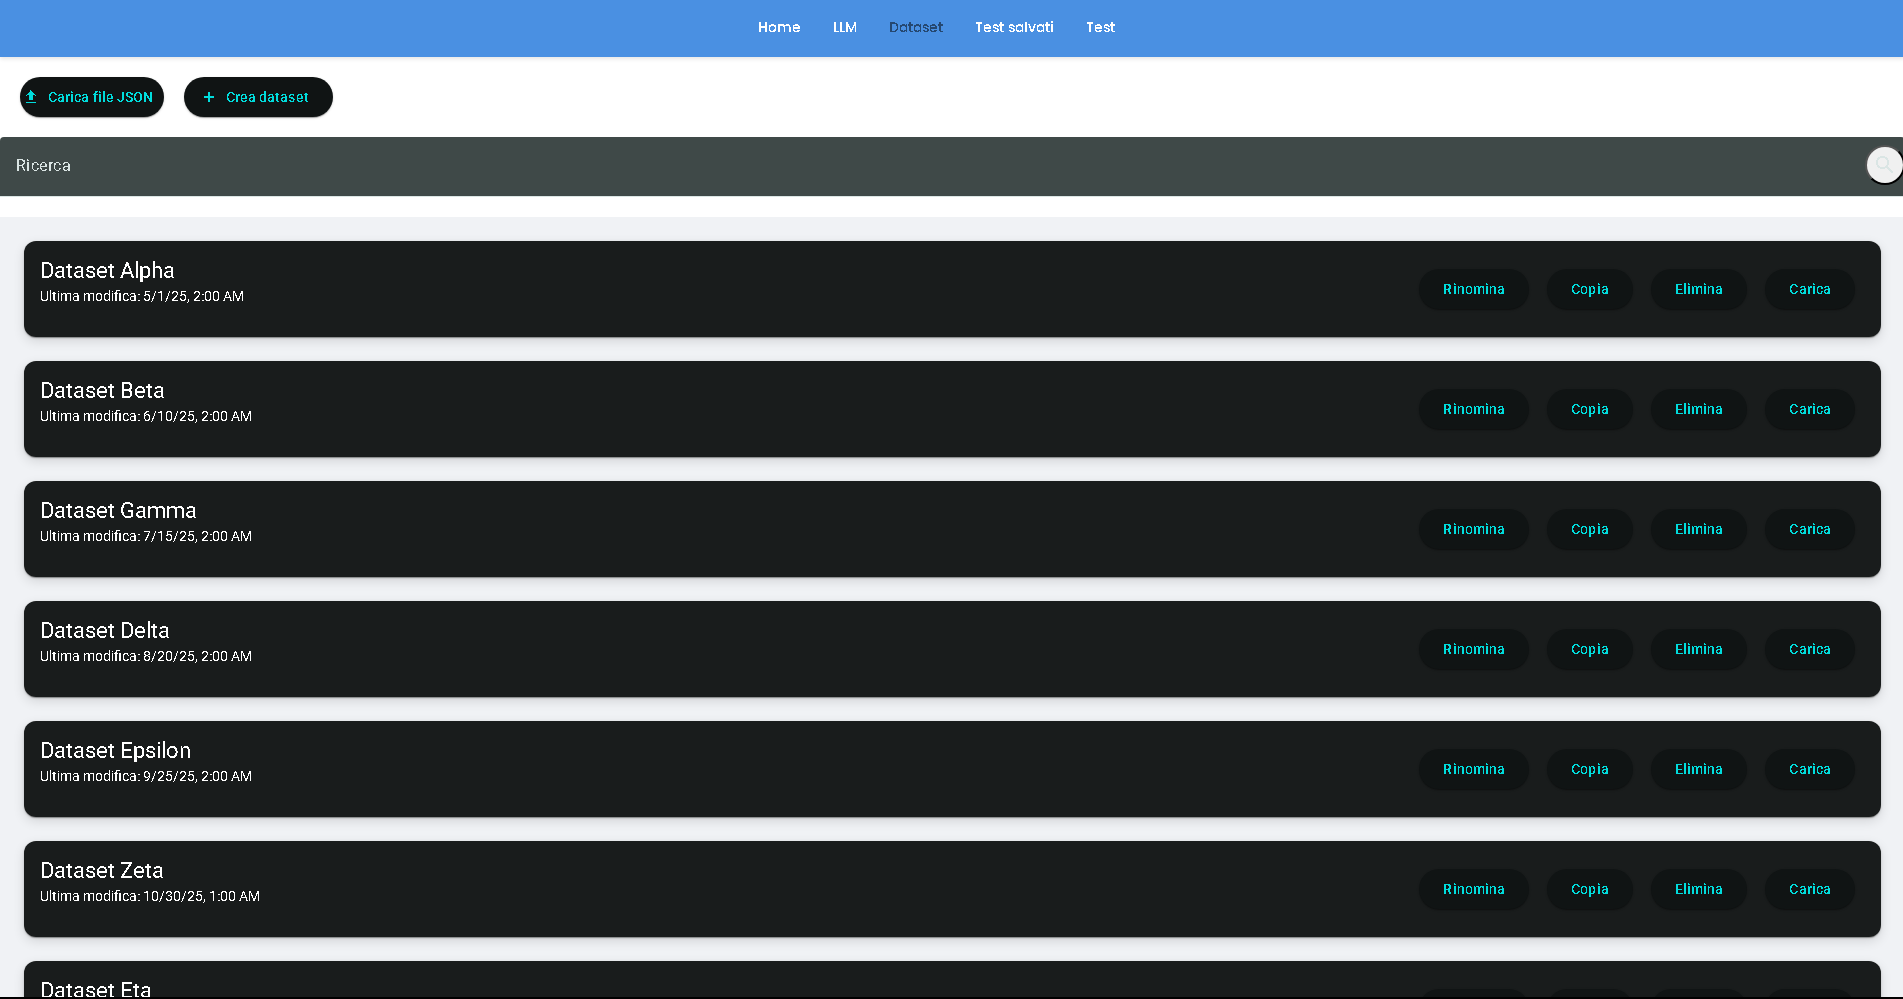
\includegraphics[width=0.25\linewidth]{Immagini/Dataset_Page.png}
\caption{\label{fig:datasets}Schermata per la gestione dei Dataset.}
\end{figure}

\subsubsection{Search Bar}
Permette un filtraggio preciso dei vari dataset caricati dal database.
\begin{figure}
\centering
\includegraphics[width=0.25\linewidth]{Immagini/SearchBar_Dataset_Option.png}
\caption{\label{fig:searchbar_dataset}Opzione per la ricerca dei dataset.}
\end{figure}

\subsubsection{Rename dataset button}
Consente di rinominare il dataset mostrando un form per l'inserimento del nuovo nome.
\begin{figure}
\centering
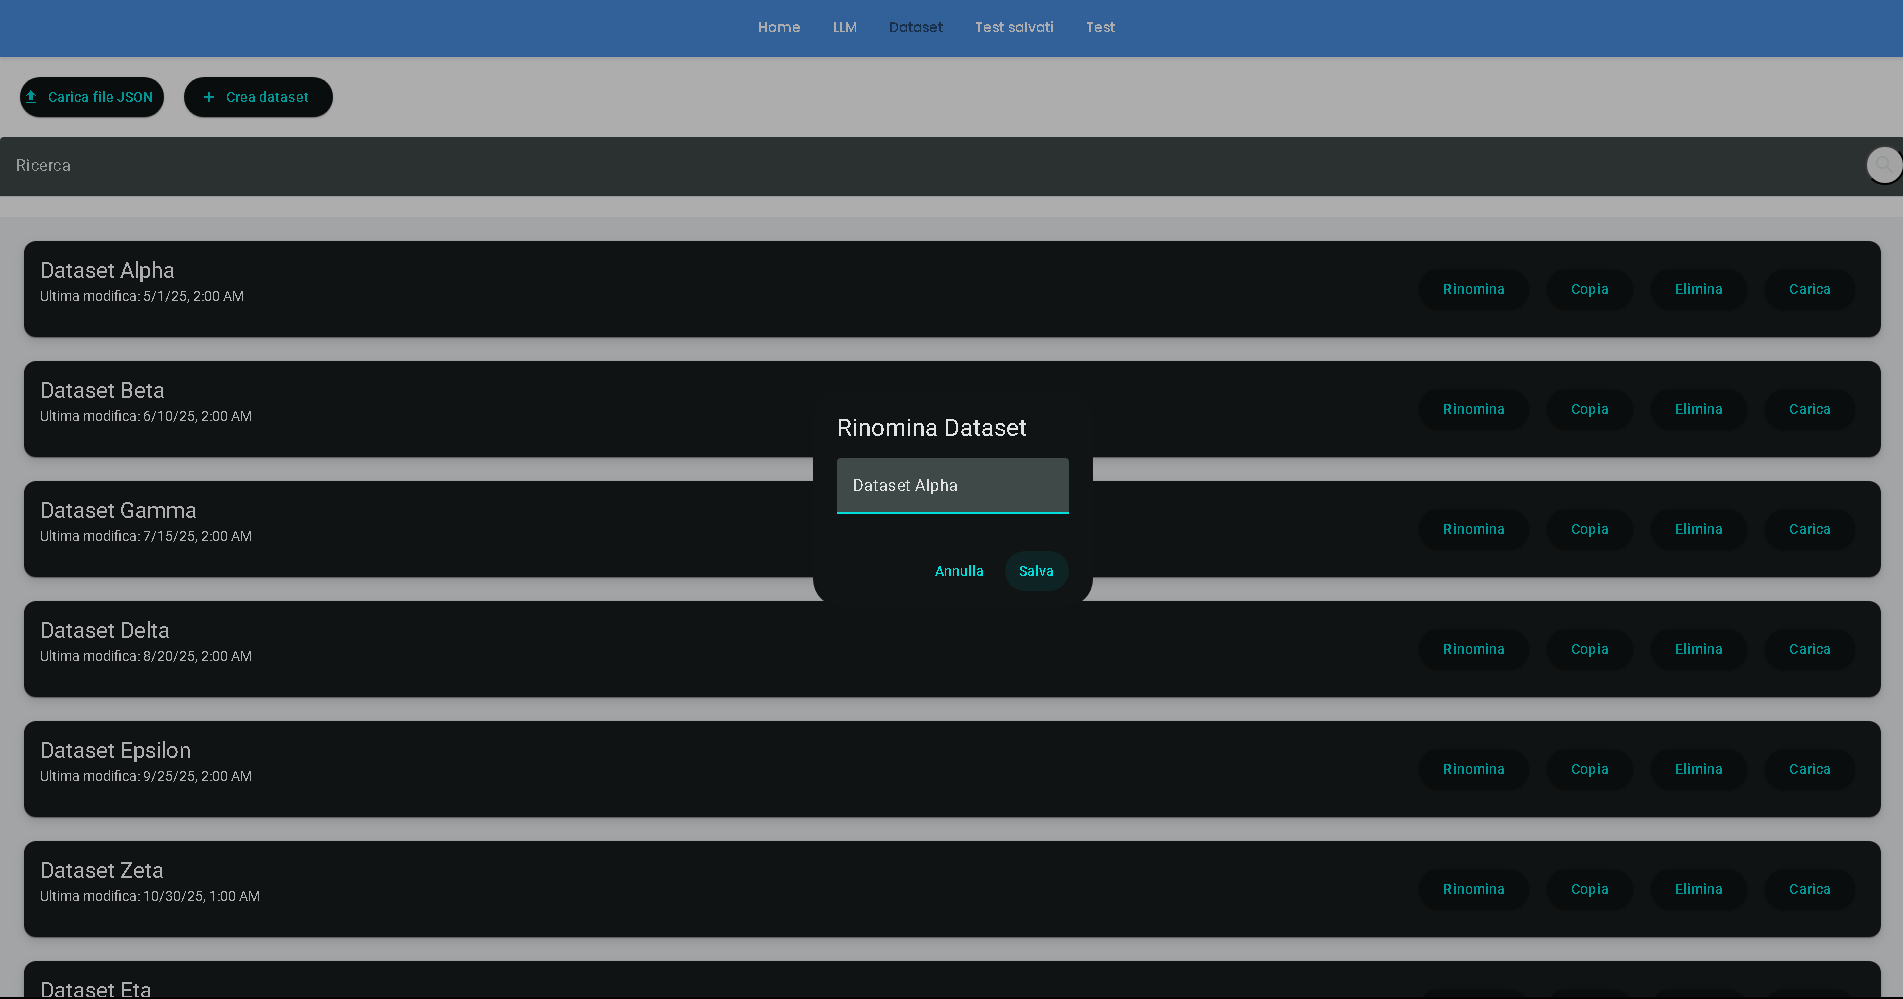
\includegraphics[width=0.25\linewidth]{Immagini/Rename_Dataset_Option.png}
\caption{\label{fig:rinomina_dataset}Opzione per la rinomina di un Dataset.}
\end{figure}

\subsubsection{Copy dataset button}
Consente di duplicare il dataset aggiungendone uno nuovo alla lista nella pagina corrente con lo stesso nome del dataset copiato con, in aggiunta un "\(1\)" alla fine del nome.
\begin{figure}
\centering
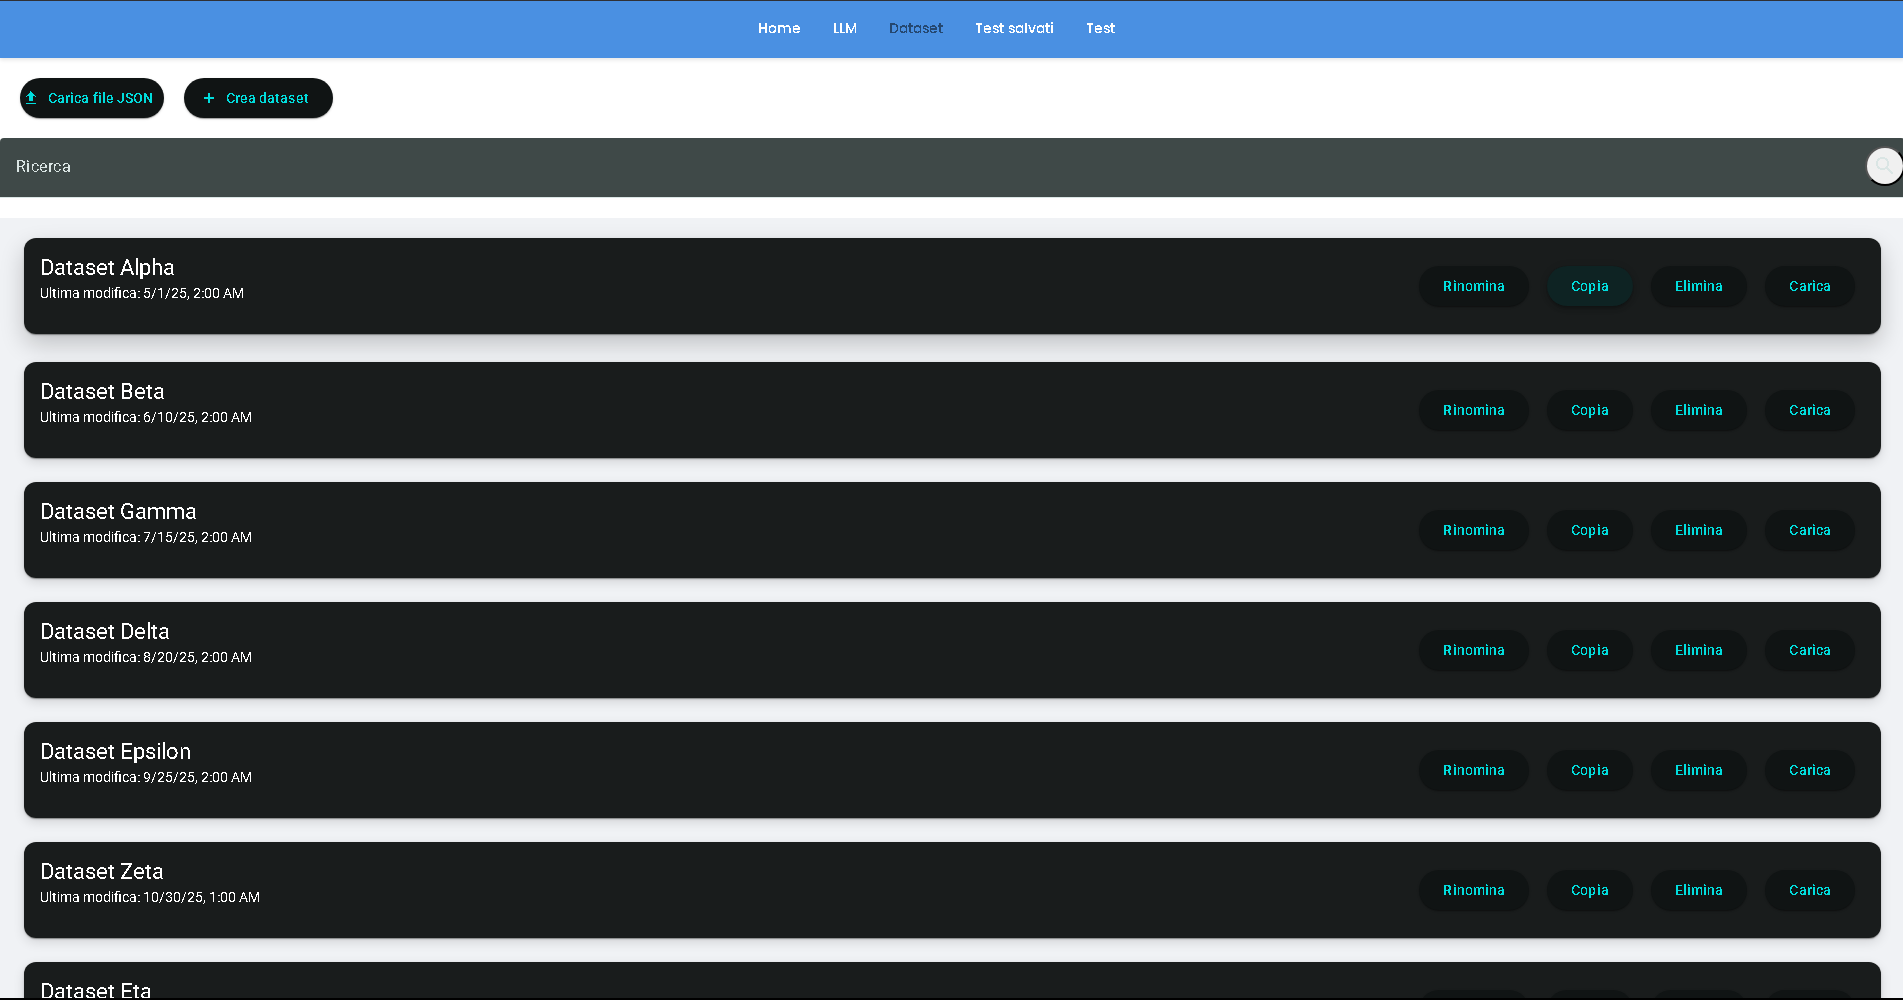
\includegraphics[width=0.25\linewidth]{Immagini/Copy_Dataset_Option.png}
\caption{\label{fig:copia_dataset}Opzione per la copia di un dataset.}
\end{figure}

\subsubsection{Delete dataset button}
Consente l'eliminazione dalla lista corrente e dal database del dataset.
\begin{figure}
\centering
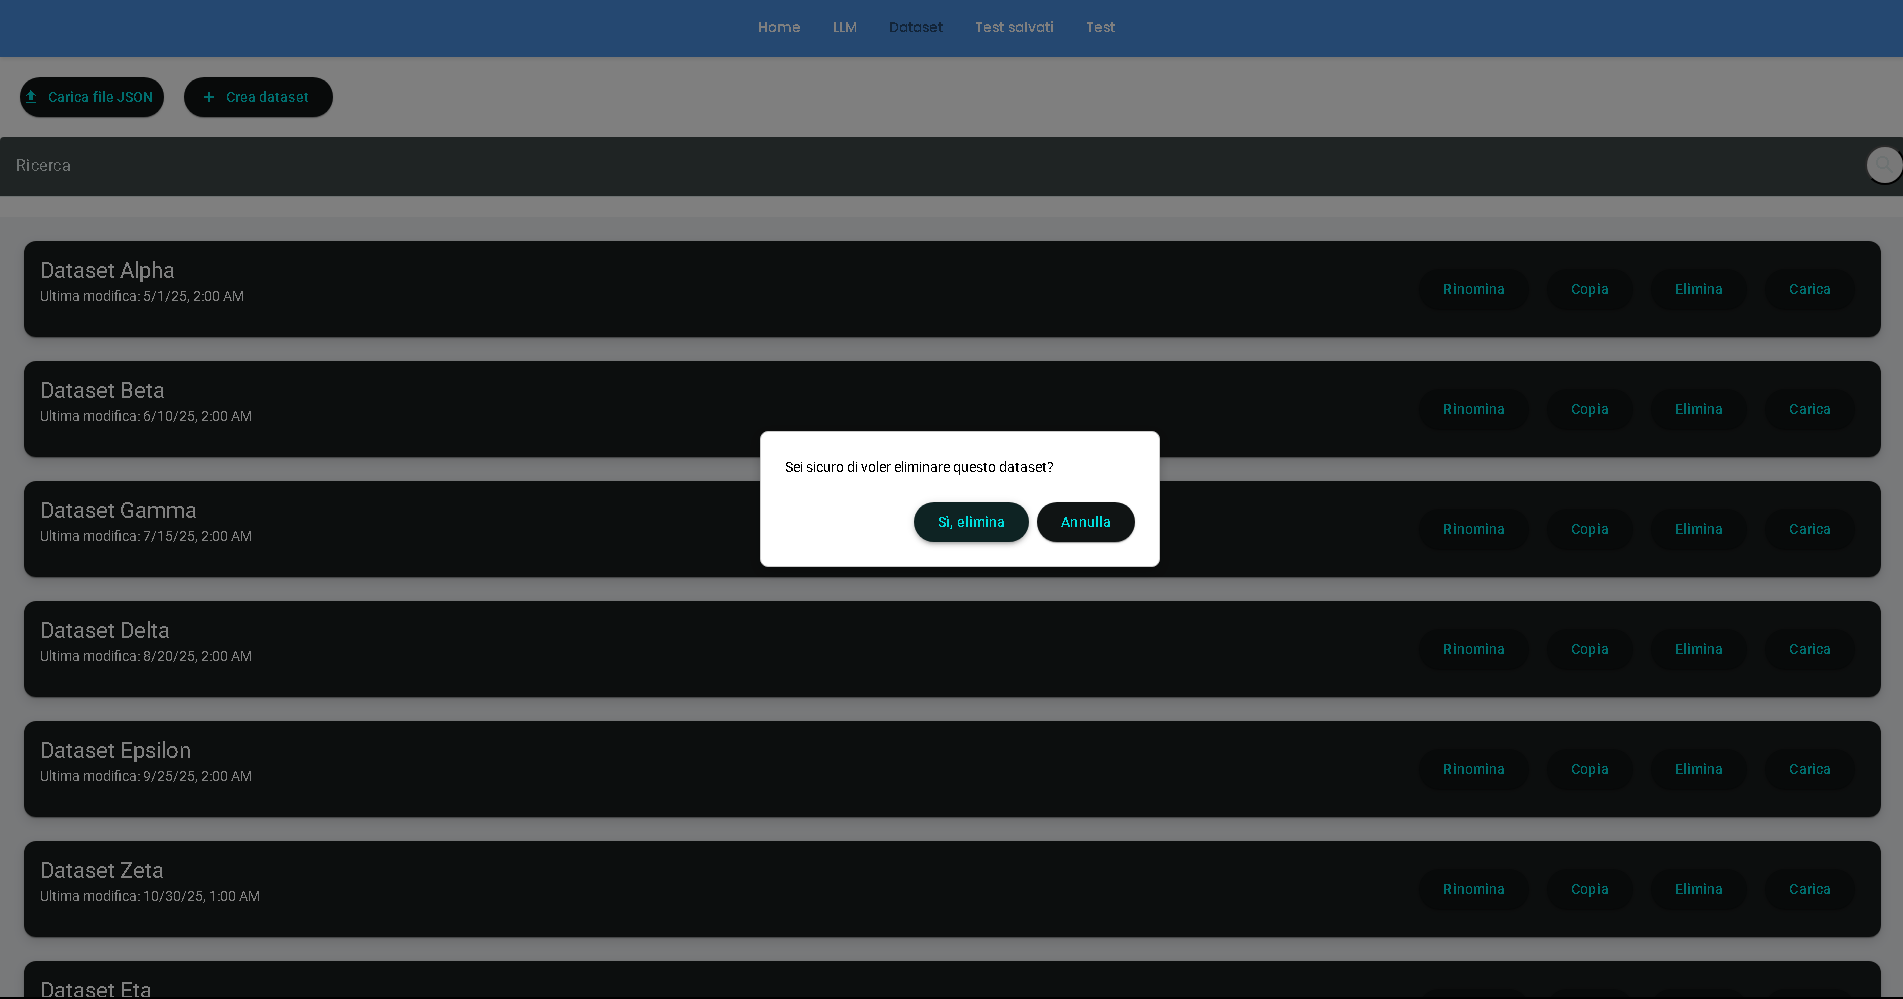
\includegraphics[width=0.25\linewidth]{Immagini/Delete_Dataset_Option.png}
\caption{\label{fig:eliminazione_datasets}Opzione per l'eliminazione di un dataset.}
\end{figure}

\subsubsection{Load dataset button}
Consente il caricamento in memoria del dataset, aprendo la pagina relativa al dataset con le informazioni relative.
\begin{figure}
\centering
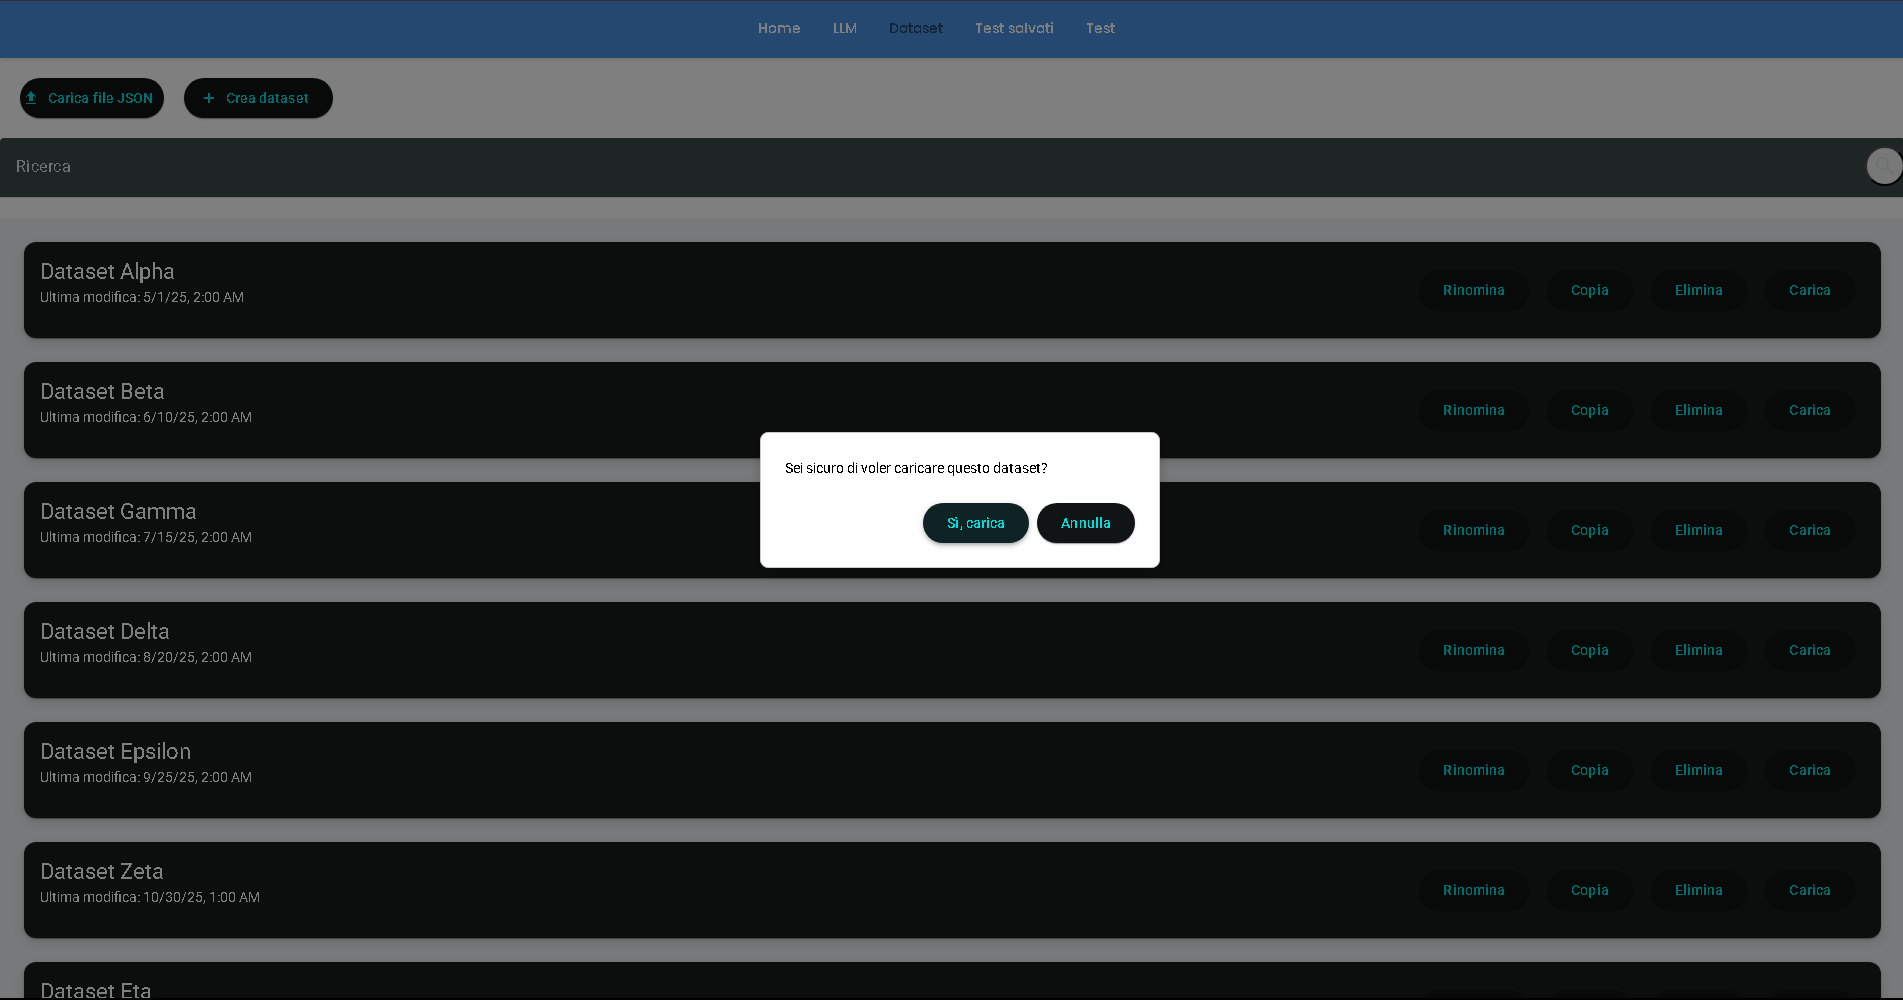
\includegraphics[width=0.25\linewidth]{Immagini/Load_Dataset_Option.png}
\caption{\label{fig:caricamento_datasets}Opzione per il caricamento di un dataset.}
\end{figure}

\subsubsection{Load from json dataset button}
Consente di caricare un file json per la creazione di un dataset.
\begin{figure}
\centering
\includegraphics[width=0.25\linewidth]{Immagini/Load_Dataset_from_json_Option.png}
\caption{\label{fig:caricamento_json_datasets}Opzione per il caricamento di un dataset da json.}
\end{figure}

\subsubsection{create dataset button}
Apre una nuova pagina dedicata alla creazione di un dataset nuovo.
\begin{figure}
\centering
\includegraphics[width=0.25\linewidth]{Immagini/Create_dataset_Option.png}
\caption{\label{fig:creazione_datasets}Opzione per il caricamento di un dataset.}
\end{figure}